\contribution{The Vector Fetch Unit}
\shortcontributor{CS6230 : CAD for VLSI Project Report}
\shortcontribution{Vector Extensions}
\headnum{7}
\begin{paper}
\renewcommand*{\pagemark}{}

\section*{}
The vector accelerator's degree of parallelism is upper bounded by the width of the data bus. The fetch unit breaks down a vector into parts of this size and get the data from memory sequentially. The data request is made through the Memory access Control Unit. For instance, suppose the data bus's width is 512 bits, and the vector units can support 512 bits; the degree of parallelism is 64 elements for 8-bit ints, 32 elements for 16-bit, and 16 elements for 32-bit floats \& ints. The fetched data is enqueued to a temporary storage unit from where the data goes to a pipelined execution unit.

\section*{Temporary Storage Units\sdot}
\begin{figure}[H]
\centering
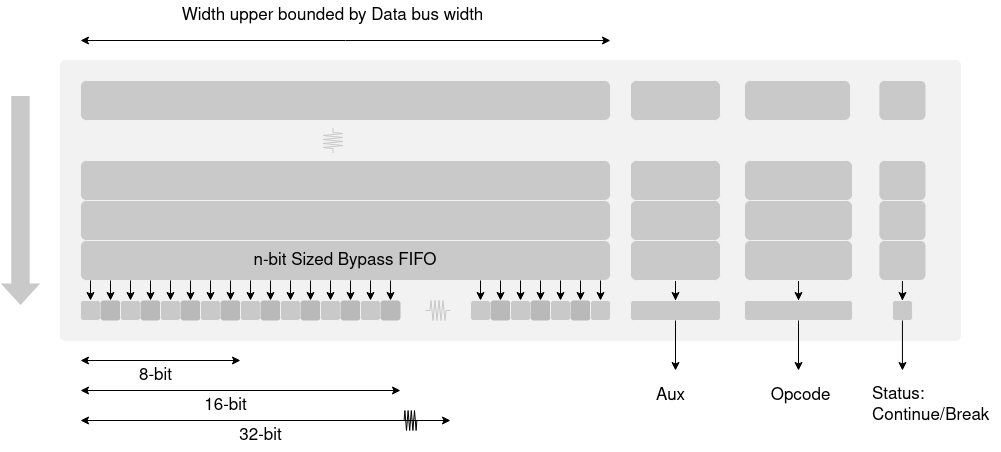
\includegraphics[width=\textwidth]{Images/VectorExtensions-temp_structure(2).png}
\caption{\content Structural view of the temporary storage units}
\end{figure}\\
\nointend The temporary storage unit is constructed out of Bypass FIFOs. Bluespec does not support the construction of sized Pipeline FIFOs, but similar functionality can be obtained by having a Pipeline FIFO in series with a sized Bypass FIFO. The outputs can be deciphered according to the Opcode and can be gathered by the appropriate execution unit. The width of the complete unit depends on the highest bandwidth supported through the bus. The functional representation of such a unit is manifested in the following figure.
\begin{figure}[H]
\centering
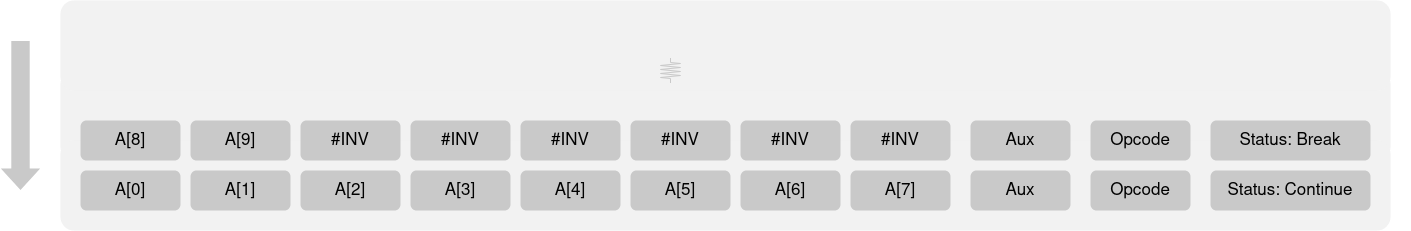
\includegraphics[width=\textwidth]{Images/VectorExtensions-temp-func(1).png}
\caption{\content Functional view of a 64-bit wide storage unit storing a vector of int8 A[10]}
\end{figure}


\end{paper}